
\documentclass{kuisthesis}


\usepackage{float}
\usepackage{color}
\usepackage{multicol}
\usepackage[dvipdfmx]{pict2e}
\usepackage{graphicx}
\usepackage{ulem}
\usepackage{amsmath,amssymb}

\jtitle[警備員ロボットの抑止力向上のためのオペレータ支援システム\\に関する研究]{警備員ロボットの抑止力向上のための\\オペレータ支援システムに関する研究}
\etitle{Study on Operator Support System for Improving Deterrence of Security Robot}
\jauthor{天野 岳洋}

\eauthor{Takehiro Amano}
\supervisor{神田 崇行}
\date{2024年1月31日}
\begin{document}
\maketitle
%=====================================================================================

\begin{jabstract}


アバターロボットが普及しアバターを介して遠隔地から勤務することが新たな働き方として認められつつある。
例えばスタッフ全員がアバターロボットのカフェ「分身ロボットカフェDAWN」であったり、
ugo株式会社による警備アバターロボットugoの、ミツカングループや東北電力株式会社といった企業での導入例などがある。
リモートワークは通勤の必要がないことや、ワークライフバランスの向上などの様々な面で優れているが、ミーティングアプリによる従来のリモートワークでは
物理的作業を伴った業務を行うことは困難であった。
アバターロボットはそのような業務であっても、リモートワークを可能にすることが大きなメリットであり、
今後ますます普及することが予想される。また様々な業務の中で重要とされる注意という行為において、
ロボットを介して行うことで、注意した相手とのトラブルを避けることができることも長所としてあげられる。
しかし、ロボットによる注意には大きな問題点もある。
それはロボットの操作が難しいことと、注意したときに相手にその行動をやめさせる力、抑止力が欠如しているというものである。
本研究では以降、アバターロボットを用いて警備員業務を行う際の歩きスマホを注意するシチュエーションを考え、
その際にオペレータを支援するシステムの開発を行う。

移動に関してロボットの歩行速度や人との遠近感をつかみづらいなどの理由から、
予備実験では7人がロボットの近くで歩きスマホをしていたのに対し、実際に相手の視界に入って注意を行えたのは2人であった。
そこでオペレータ支援のためにまず移動支援システムの開発を行った。これによって、オペレータは画面上で人をクリック
するなどの簡単な操作でその人の前までロボットを移動させ、できる限りその人に追従させることが可能になった。

次に抑止力の向上に有効な注意文言についての検討にあたって、
人が歩きスマホを注意されてもやめない人がいる理由を次のように仮定した。
注意されたことで「歩きスマホは危険である」という信条と、「自分は歩きスマホをしている」という行動に関する認知とが矛盾することに気づかされ、
その認知の矛盾によって不快感が生じ、その不快感の解消のために行動をやめる。
しかしこの時
行動をやめる以外にもこの不快感を解消する方法が3種類存在するため、
歩きスマホをやめない人がいる。そこで、注意された人がどのような方法で不快感を解消したかを
推定し、その解消方法に対抗する文言によって不快感の解消を難しくすることで、
行動をやめさせることが可能になるつまり抑止力が高まるのではないかと考え、
それぞれの解消方法に対抗する文言を考案した。それは歩きスマホの危険性を強調するもの、
相手の言い逃れを防ぐもの、そして相手を特定するものである。

しかし現段階ではオペレータに相手の解消方法を推定することが求められており、
これは認知的不協和理論についての知識や相手の行動に対する洞察が必要となる。
そのためどのような行動のときどの解消方法がとられたのか、
その注意文言は実際に有効なのかを明らかにするために
ATCというショッピングモールにて実験を行った。
事前に協力をお願いした2人の参加者に対して注意されたときにどのように感じたかのアンケートを、
また歩きスマホをしていた5組のATCへの来客者に対して注意を行ったときの反応の観察を行なった。アンケートでは
相手を特定する文言では、自分だけが注意されているという孤立感を感じ周囲の圧力を感じることで無視することが難しくなった
という意見が得られた。また実際の観察では、歩行速度やグループの人数といった属性の値によって解消方法を推定することができる可能性が示唆された。

以上のように本研究では、移動操作の支援を行うシステムの開発と解消方法ごとの有効な文言の検討を行った。
また実験からはいくつかの値から解消方法の推定が行える可能性が示唆された。今後、さらなる実験を行い解消方法の予測モデルを構築することで、
オペレータに有効な文言を提示するシステムの構築が課題となる。またアンケートの結果から、
同調圧力によって歩きスマホをやめさせることができる可能性が考えられる。そのため、
同調圧力を用いた戦略を取り入れたシステムの構築も将来課題として考えられる。
\end{jabstract}


\begin{eabstract}
Avatar robots are becoming more and more popular, and working remotely through avatars is becoming a new way of working.
For example, there are the avatar robot cafe "Bunshin Robot Cafe DAWN" or the security avatar robot ugo by ugo Co., Ltd. whose introduction to companies such as Mitsukan Group and Tohoku Electric Power Co., Ltd.
Remote work has many advantages, such as no need to commute and improved work-life balance, but with the conventional remote work using meeting apps, it was difficult to do physical work.
Even in such work, avatar robots have the great merit of making remote work possible, and it is expected to become more and more popular in the future. 
Also, in the the act of admonishing that is considered important in various works, it is also a merit that can avoid trouble with the person who was warned by the robot.
However, there are also major problems with the admonishing of robots.
One is that the operation of the robot is difficult, and the other is that the robot lacks the power to stop.
In this study, we assume a security avatar robot and consider a situation where warn a person using a smartphone while walking, 
and develop a system to support the operator in such a situation.

Regarding movement, it was difficult to grasp the walking speed of the robot and the sense of distance from the person, and in the preliminary experiment, while there were 7 people who were walking and watching the smartphone near the robot, only 2 people were actually warned in the person's field of view.
Therefore, we developed a movement support system for operator support. With this system, the operator can move the robot to the front of the person with a simple operation such as clicking on the person on the screen, and can follow the person as much as possible.

Next, we assumed that when a person is warned about walking and watching a smartphone, he or she realizes that the cognition that "walking and watching a smartphone is dangerous" and the cognition that "I am walking and watching a smartphone" are contradictory, and that the contradiction in cognition causes discomfort, and that he or she stops the behavior to resolve the discomfort. According to the cognitive dissonance theory, there are three main ways to resolve this discomfort other than to stop the behavior. Therefore, we devised a warning phrase to counteract each of these methods, which are to emphasize the danger of walking and watching a smartphone, to prevent the other person from escaping, and to identify the other person. However, at the present stage, it is required that the operator estimate the other person's method of resolving the discomfort, which requires knowledge of cognitive dissonance theory and insight into the other person's behavior.

Then, in order to clarify how each action was taken and whether the warning phrase was actually effective, we conducted an experiment at ATC, a shopping mall. We conducted a questionnaire on how the two participants who had been asked for cooperation felt when they were warned, and observed the reactions of five pairs of ATC visitors who were walking and watching smartphones. In the questionnaire, it was found that when the other person was identified, it was difficult to ignore the warning because of the feeling of isolation that only he or she was warned and the feeling of pressure from the surroundings. In the actual observation, it was suggested that the method of resolving the discomfort could be estimated from the values of walking speed and the number of people in the group.

In this study, we developed a system to support the operator's movement and examined effective phrases for each method of resolving the discomfort. In addition, the experiment suggested that it is possible to estimate the method of resolving the discomfort from several values. In the future, it will be a challenge to build a prediction model of the method of resolving the discomfort by further experiments and to build a system that presents effective phrases to the operator.
In addition, from the results of the questionnaire, it is possible that the reason for stopping walking and watching a smartphone is not only to resolve the discomfort, but also to conform to the pressure.
Therefore, it is also a future task to compare these two strategies and examine a strategy that combines them.
\end{eabstract}
%=====================================================================================

% 目次の表示
\tableofcontents


%=====================================================================================
%=====================================================================================

\section{はじめに} %章

\subsection{研究背景} %1.1
%アバターロボットについての説明a
アバターロボットとは人間が遠隔地からロボットを操作することで、
人が実際にその場所に行くことなく現地での作業を可能にするロボットのことであり、
そのロボットを介して遠隔地から作業を行うことをテレオペレーションと呼ぶ。
この性質からアバターロボットは、
それまで難しかった物理的な作業を伴うサービス業や飲食業などの分野におけるリモートワークを可能にする。
例えばugo株式会社\footnote{https://ugo.plus/}によるアバターロボットugoは、
ビルメンテナンスや警備業務のためのアバターロボットであり、
トイレ清掃や警備、巡回等の業務を遠隔地から行うことができる。
リモートワークは働く場所を問わないことから通勤の必要がないことや、ワークライフバランスの向上、
時差を利用した業務が可能になることなどの長所があげられる。
加えて他の人間と直接接する機会が少ないことなどから、
パンデミック時において感染を心配する必要がないことも大きなメリットである。
実際にアメリカでは2020年の新型コロナウイルスの流行によって、
それまでは従業員のうちリモートワークをしている割合は約13\%だったが、
2020年の4月にはおよそ56\%から74\%に増加した\cite{ozimek2020future}。
またリモートワークは従業員だけでなく企業にとっても利点があることがわかっている。
例えば\cite{FERREIRA202170}では、企業が地理的制約なしに優秀な人材を獲得できることや、
オフィスの維持費や交通費を削減できることがあげられている。

他にも身体障碍を持つ人がアバターロボットを用いることによって、
カスタマーサービスといった業務を行うことができるようになる。
さらにその際に、身体障碍を持つ人の社会参加感や精神的充足感をもたらすことがわかっている\cite{takeuchi2020avatar}。
アバターロボットは自律ロボットでは難しかった人との柔軟なコミュニケーションが可能である。
現時点で自律ロボットは人の表情や声のトーン、仕草などを読み取り相手の感情を推測することが困難であることや、
音声認識の問題などから人とのコミュニケーションにおいて限界があるが、
一方でアバターロボットでは人が操作するため、人とのコミュニケーションにおいて自律ロボットよりも柔軟な対応が可能である。
これらのことから、アバターロボットを介したリモートワーク業務は教育、介護、サービス業等の分野で広く普及することが予想される。

今後アバターロボットが担うであろう様々な業務において人々を注意し、
特定の行動を抑止するという行為は重要である。
例えば、教育の場面において先生は生徒が集中力に欠く行動をとっていたとき、
注意することによってその行動をやめさせ生徒の集中を取り戻すことができる。
またサービス業の場面においては、
他の客に迷惑をかける行動を取る客がいたときに店員が注意することで、
その行動をやめさせ他の客の満足度の低下を防ぐことができる。
しかし、人を注意するという行為には逆上した注意相手とのトラブルに陥るかもしれないといったリスクも伴う。
ロボットを用いた場合、注意相手との直接のコミュニケーションが存在せずそのようなリスクが小さいことから、
ロボットは注意を行う際の便利なツールとなる。
以上のことから、アバターロボットを介した業務の中で注意という行為は重要な役割を果たすことになる。

しかしロボットによる注意にも人間による注意とは異なった問題点もある。
それは移動操作の困難性と抑止力の欠如である。
ここで本研究では抑止力を歩きスマホのような社会的規範に背くような行動をしている相手に対して
注意を行ったときに、その行動をやめさせる力と定義する。

移動操作に関して、
ロボットの最大移動速度は安全のために通常の人の歩行速度より低めに設定されていることや、
ロボットからのカメラ映像では空間認識が困難であることから、
移動操作が難しくそもそもその人の視界に入ることが難しい場合がある。
実際に予備実験では、%DUALSHOCK4及びキーボードを用いてロボットを操作し、歩きスマホをしている客への注意を行ったところ、次のような移動に関する問題があることが分かった。まず、注意を効果的に行うためには相手の視界に入り続けさらにロボットが相手の方向を向いている必要がある。そうでないと多くの場合注意された人は自分が注意されているとは気づかず無視される結果となったからである。人の視界内に立つためには人の将来いるであろう位置にロボットを移動させる必要がある。そのためロボットはその対象の現在位置ではなく予測位置をむくことになり、結果その人をロボットのカメラの視野から外す必要があった。しかし、それでは今その人がどこにいるかわからないまま、おそらく来るであろう位置に移動を続けなければならない。また人と対話できる距離まで追いつけたとしても、その人と対面するためにロボットの向きを変える必要があった。これらの操作はDUALSHOCK4、キーボードのいずれでも困難であり操作に集中する必要があったために、十分に相手との対話や相手のしぐさに集中できなかった。
その人の視界に入るまでの移動やその人の視界に入った後の追従の操作が難しく、相手に気づいてもらえないことや
対話に集中できないことが問題となった。
またほかにも歩きスマホをしている人を探すためにいろいろな方向にロボットを向ける必要があり、
常にロボットを回転させなければならなかったため、歩きスマホをしている客を見つけるまでに
時間がかかり、見つけた時にはすでに追いつけない距離にいることもあった。
その結果、予備実験の中で歩きスマホをしている客がロボットの近くを通った回数は7回あったが、
そのうち相手の視界に入って注意を行えたのは2回であった。

抑止力に関して例えば\cite{Schneider2022}では、歩きスマホをしている人に対してロボットが二回にわたって
「歩きスマホ危険ですからおやめください」と注意を行った時に、
160人中76人が1回目の注意を無視し、さらにそのうち72人が2回目の注意も無視したという結果が得られている。
これに関して同論文では、注意を無視した人のインタビューの結果から、
ロボットが人間らしくないことで注意された際に実際に人間に注意されているとは感じず、
たかがロボットに注意されているという認識を持つことが多いためであると考察されている。

アバターロボットを介した業務の普及が予測される中で、
注意時における移動操作の困難性と抑止力の欠如は重大な問題である。そこで本研究では
これら二つの課題に取り組む。


\subsection{研究手法}
\label{sec: 研究目的}
本研究では、アバターロボットが抱える問題である移動操作の困難性と抑止力の欠如を解決するために、
移動操作支援を行うシステムの開発と有効な注意文言の検討を行った。
有効な注意文言を考えるにあたって、
人が規範に反する行動を注意された時その行動をやめる理由として、以下のように仮定した。
まず注意されることによって自らの信条と自らの行動に関する認知とが矛盾することに気づかされる。
そして認知的不協和理論\cite{Festinger1957}に基づきその認知の矛盾によって不快感がうまれ、
その不快感の解消のために注意された行動をやめると仮定する。
しかしこの不快感の解消は行動をやめること以外によっても可能であるため、
注意をされても行動をやめない人がいると考えられる。
そこで抑止力向上のために、
それらの解消方法に対抗するいくつかの注意文言を考えた。
その後開発した移動支援システムを用いて実際のフィールドにて実験を行い、
どのような場合にいずれの注意文言が効果的であるかを明らかにすることを目標とした。
これが明らかになれば、有効な注意文言としてあり得るものの提示や、
どのような状況下ならばどの注意文言が有効かについての知識の提示を行うシステムの開発が可能となり、
業務パフォーマンスの向上につながると考えられる。


本研究では以降、アバターロボットが注意するシチュエーションとして警備員アバターロボットを想定している。また簡単のために
注意すべき行動を\cite{Schneider2022,Mizumaru2019}と同じように歩きスマホのみとした。これは、歩きスマホがもっともよく観測される
迷惑行為であり、実際にやめたかどうかを確認することが容易であるためである。



\section{関連研究}
このセクションでは、HumanRobotInteraction(HRI) における認知的不協和理論を適用した研
究を紹介する。その後歩きスマホを注意しやめさせるといった、人の行動に影響を与えるた
めに否定的なフィードバックや行動をとるロボットに関する研究について紹介を行う。そして開
発するシステムのようなテレオペレーション支援に関する研究について様々な例と本研究との差
異について説明を行う。
\subsection{認知的不協和のHRIへの適用研究}
HRI分野における認知的不協和理論の適用例を示す。例えば研究\cite{washburn2022exploring}では、
人間が荷物配達ロボットに対して従順になる理由の説明として、認知的不協和理論を用いている。具体的には、
人間がロボットにタスクを依頼された場合に、人間が「タスクを果たすことを楽しいことだ」という認知を追加する傾向があることを
人間がロボットに対して従順になりやすいことの説明としている。また他にも研究\cite{herse2018you}では、ロボットがわざと
最適ではない選択肢を人間に提供した際に、信頼されているロボットのほうがそうでないほうよりも、人間が反応を返すまでに
長い時間がかかることが示されている。この理由として
人間がロボットを信頼している場合ロボットが不適切な選択肢を提示した際に、
不協和が生じ意思決定時に余分な負荷がかかるために、反応時間が長くなるという説明を行っている。
しかし、これらのように多くの研究は、
あくまで結果の説明のために認知的不協和理論を用いているものであり、
ロボットがとるべき戦略を決定するために用いているものではない。

認知的不協和に基づく不快感を戦略として利用した歩きスマホの注意を行っている研究は存在している\cite{Schneider2022}。
しかし上記研究では自律ロボットを前提としているため注意された時に生じる不快感の解消方法として、
どのようなものが用いられているかのその場での分別は難しいものとしており、行動をやめるか、ロボットの矮小化を行うことを仮定している。これは
注意を無視した人のアンケートで、歩きスマホを行っている人が注意された際に用いる「行動を変える」以外の不快感の解消方法として、
ロボットの矮小化が多かったためである。ロボットの矮小化とは例えば、
ロボットが機械音声を用いているために、ただのガイダンスだと捉えられたや、ロボットがただの機械であると捉えられたなどである。
そのため、一度単に「歩きスマホは危険なのでおやめください。」と注意されたが引き続き歩きスマホを行っている人に対して、
「あなたは私のことをただのロボットだと思っているかもしれませんが、私はみなさんのために働いているのです」と一律に話しかけることによって、ロボットの矮小化
を防ぐことを試みている。一方で本研究ではアバターロボットを用いており、オペレータとして人間が操作することを前提としているため、
より柔軟な戦略を取ることが可能である。そこで、使用されたであろう解消方法に基づいて異なる文言を提示することで、より効果的な注意を行うことができるのではないかと考える。

\subsection{説得のために否定的な行動をとるロボット}
まずはじめに説得は人の行動になにかしらの影響を与えるために行われるものであり、
本研究で取り組む抑止は特にその中でも、
特定の行動をやめさせるための説得行為を指すものとする。
ロボットがいかにして人間に対する説得力を向上させることができるかについては多くの先行研究で取り組まれている。
例えばロボットが人間とのじゃんけんゲーム内でわざと負けることによって贈賄を行い、
その後人間がロボットにお願いされた追加のタスクを行うかどうかについての研究\cite{sandoval2016can}では、
ロボットがわざと負けた場合に(贈賄を行った場合)より好感度が高く、
しかし、追加のタスクについてはより非協力的になることがわかっている。また、他にも仮想的な洗濯作業中に省エネを促す際、エネルギーをより使う設定に変えた際に、怒りの表情や批判的な言葉または不快な音といった否定的なフィードバックをとるほうが、
エネルギーを節約する設定に変えたときに、褒めるや喜びの表情を見せるといった肯定的なフィードバックよりもより効果的に人間に行動の変容をもたらすことがわかっている\cite{Midden2009}。
また研究\cite{paradeda2019makes}では、被験者が自律ロボットから助言を受けながら決断を下すようなシチュエーションにおいて、ロボットが怒り等の負の感情を
表現すると、被験者はロボットのアドバイスに従う可能性が高くなり、説得が効果的になることが報告されている。しかし、
一般的にどのようなフィードバックが最も説得力があるかという研究課題に対する明確な答えはなく、それは実験のシチュエーションや人間と
ロボットの関係性によって異なる。多くの研究では、事前に定められた二つのフィードバック手法を比較してどちらがより
効果的かどうかについて調査しており、ロボットのフィードバックに対する人間の反応によって、その後のロボットの行動を
変化させる戦略をとるような研究は少ない。そこで本研究では、相手のとった行動に対して次の発言内容を決定するような柔軟な戦略についての研究を行う。
\subsection{テレオペレーション支援に関する研究}
テレオペレーション支援に関する研究は多く行われており、様々な面から種々のシステムが開発されてきた。
例えば\cite{chen2007human,triantafyllidis2020study}では、テレオペレーションにおいて課題となっている視野の狭さや方向感覚の喪失といった問題を、
視覚だけでなく聴覚や触覚などの他の感覚を利用する多モーダルインターフェースによって解決を試みている。
また、多数の無人航空機を操作する際にパフォーマンスを向上させる
ようなコントローラーへのハプティックフィードバック手法についての研究\cite{son2011measuring}などがある。
へパティックフィードバックとは、コントローラーの利用者に力や振動によって警告等を行うフィードバック手法のことである。
他にも鉱業において採掘を行うロボットのテレオペレーションでの
ユーザーインターフェースについての研究\cite{hainsworth2001teleoperation}や、
テレオペレーターが荒い言葉遣いで話したとしても意図認識を用いて、支援システムが丁寧な言葉遣いに変換するような支援システム\cite{Daneshmand2023}などいろいろなものが研究されている。
しかし、これらの研究のように大半では操作や発言を行いやすくするための支援に関する研究であり、
それらの操作内容や発言内容は操作者が決定しなければならず、オペレーターは
どういった操作、どういった発言が効果的かを考える必要がある。
そこで本研究では
警備員業務の中で注意時に必要な知識をオペレータに提示し、
オペレータは
自分でどのようなものが有効か考える必要なく有効な注意喚起を行うことが可能になるような
支援システムの開発を目標とする。

\section{認知的不協和とは} %1.1.2
\label{sec: CDT}
この章では、人が注意されたときに不快感が生じる理由とその不快感の解消方法の説明のために、
認知的不協和理論について紹介を行う。
認知的不協和理論\cite{Festinger1957}とはFestingerにより提唱された理論であり、人間が互いに相反する認知を抱いた場合、その状態(不協和)に不快感を感じ
その不快感の解消のために、不協和の解決を図るというものである。
この認知とは、行動、知覚、態度、信念、感情といった様々な事象に関するものであり、多くの場合片方の認知は自らの行動に関するものである。
例えば、表\ref{fig: CDTExample}のようにたばこは健康に良くないと分かっているのに、タバコを吸ってしまった際に生じる不快感が認知的不協和である。
この不快感は、認知1と認知2が矛盾しているために生じるものである。
\begin{table}[H]
  \centering\caption{認知的不協和の例}
  \label{fig: CDTExample}

  \begin{tabular}{c|c}
      認知1 & たばこは体に害をもたらす  \\ \hline
      認知2 & 私はたばこを吸っている \\ 
  \end{tabular}
  
\end{table}
この不快感を解消するために、「行動を変える」「認知を変える」「新たな認知の追加を行う」「矛盾の矮小化、無視」の4つの選択肢をとることができる。
それぞれについて表\ref{fig: CDTExample}のたばこの例を用いて具体的に説明を行う。
\begin{enumerate}
  \item 行動を変える \\
  行動を変えることは、たばこを吸うのをやめることであり表\ref{fig: CDTExample}の認知2の変化をもたらす。そして表\ref{fig: ReduceDissonanceAction}のように認知1と認知2の不一致を解消することができる。
行動の変更が容易なものであればこの方法をとることが最も理論的であるが、行動の変更が困難な場合もある。そのような場合
この方法ではなく他の方法をとることになる。
  \begin{table}[H]
    \centering
    \caption{行動を変える例}
    \label{fig: ReduceDissonanceAction}
    \begin{tabular}{c|c}

        認知1 & たばこは体に害をもたらす  \\ \hline
        認知2 & 私はたばこを\sout{吸っている}吸わない \\
    \end{tabular}
\end{table}
 \item 認知を変える \\
  認知を変えることは、表\ref{fig: CDTExample}の認知1を「たばこは体に害をもたらさない」とすることである。
  これにより認知は表\ref{fig: ReduceDissonanceChange}のように変化し、
  実際に行動を改めることなく認知1と認知2の不一致を解消することができる。
  \begin{table}[H]
    \centering
    \caption{認知を変える例}
    \label{fig: ReduceDissonanceChange}
    \begin{tabular}{c|c}
        認知1 & たばこは体に害を\sout{もたらす}もたらさない  \\ \hline
        認知2 & 私はたばこを吸っている \\
    \end{tabular}
    
  \end{table}

  \item 新たな認知の追加 \\
  新たな認知の追加を行うことは表\ref{fig: CDTExample2}の認知3や認知4を追加することであり、
この追加によって認知1と認知2の不一致度合いを軽減させることができるため生じる不快感が小さいものとなる。
\begin{table}[H]
  \centering
  \caption{新たな認知の追加の例}
  \label{fig: CDTExample2}
  \begin{tabular}{c|c}

      認知1 & たばこは体に害をもたらす  \\ \hline
      認知2 & 私はたばこを吸っている \\ \hline
      認知3 & \textbf{喫煙をやめると他の人にあたってしまい迷惑となる} \\ \hline
      認知4 & \textbf{たばこを吸っていて長寿の人もいる} \\ 
  \end{tabular}

\end{table}

  \item 矛盾の矮小化、無視 \\
  矛盾の矮小化、無視では認知自体を変えずに不協和を解消する方法である。このとき、注意してきた対象や
  認知同士が生む不協和が矮小化もしくは無視されることになる。例えば、そもそも表\ref{fig: CDTExample}の認知1と認知2が
それほど矛盾していないと思い込むことによって生じる不快感を軽減することができる。

\end{enumerate}
\vspace{5mm}
ここで本研究では上記方法が一つ取られた時点で、不快感が十分に解消されそれ以上の方法をとることがないことを仮定する。
従って不協和による不快感が生じた人は上記の方法のうちいずれか一つをとることになる。



\section{提案手法}
アバターロボットを用いて警備員の仕事を行うことを効率的に簡単に行うことを可能にするために、
図\ref{pic:interface}のようなインターフェースを用いて操作支援を行うシステムを開発と、
認知的不協和理論\cite{Festinger1957}に基づいた不快感の解消に対抗する注意文言の検討を行った。
この章では移動操作支援システムの詳細についての説明を行ったのちに、
認知的不協和理論に基づいた抑止力の高い注意文言について検討を行う。
また注意文言については、\ref{sec: 研究目的}節で述べたように歩きスマホに対する注意に関してのみを扱っている。

\subsection{移動操作の簡単化}
より人間らしい対話を可能にするために発話はオペレータが行う。しかしながらアバターロボットの移動操作に気をとられてしまい、
うまく対話が行えないといった問題や、そもそも話しかけることができないという問題があった。そこで、移動操作を簡単にするためのシステム及びインターフェースを開発した。
システム全体の構成を図\ref{pic:systemcompose}に示す。これらのシステムを用いることによって、オペレータは画面クリックのような
簡単な操作でアバターロボットを人の前まで移動させ可能な限りその人についていくことができるようになる。
これらの機能によってオペレータは歩きスマホをしている人に容易に話しかけることが可能になり、さらにその人の動きや反応に
集中できるようになる。
システムではデータのやり取りはROS\footnote{https://wiki.ros.org/ja}を介して行われる。ROSとは、ロボットのソフトウェア開発のためのライブラリであり
ROSを用いることで複数のプロセス間でのデータのやり取りを容易に行うことができる。
%#TODO
\begin{figure}[h]
  
  \includegraphics[width=15cm]{img/system\_compose.drawio.png}
  \caption{移動支援システムの構成}
  \label{pic:systemcompose}

\end{figure}
図\ref{pic:systemcompose}における各構成要素について説明する。
\begin{itemize}
  \item 人位置計算 \\
  既存のソフトウェアであるhuman\_trackerを利用しており、人物の位置を取得することができる。ロボットに備わったLiDARセンサーから得られた点群データと事前に作成されたマップデータを用いており、
  点群データの内からマップデータに存在しないものを人としており、その人の位置を取得することができる。また各人に対してidが割り振られ、このidは基本人に対して唯一である。
  おおよそ1秒に5回から10回ほどの頻度で人位置と人idおよびその時刻が発行され、このデータを用いて次の速度計算が行われる。
  \item 速度計算 \\
  位置の時系列データから各人idごとに速度計算を行う。速度計算では、まず人位置計算で得られた時刻、位置データをidごとに保存しておく。
  その後最大直近16個の時刻データと位置データを用いて、最小二乗法によって速度を計算している。
  具体的にX座標についての速度を求める場合、時刻とX座標の組を$(T_i, X_i)$とし$n(n <= 16)$個あるとする。この時その人の速度$V_x$は以下の式で求められる。
  \begin{equation}
    V_x = \frac{\sum_{i=1}^{n} (T_i - \overline{T})(X_i - \overline{X})}{\sum_{i=1}^{n} (T_i - \overline{T})^2}
  \end{equation}
  ここで$\overline{T}$は時刻の平均、$\overline{X}$はX座標の平均であり、次のようにして求められる。
  \begin{equation}
    \overline{T} = \frac{1}{n}\sum_{i=1}^{n} T_i, \qquad \overline{X} = \frac{1}{n}\sum_{i=1}^{n} X_i
  \end{equation}
  最大16とした理由は50等の大きい数字にすると、人の速度が変化した際に
  反応が遅くなってしまうことや計算時間の問題があり、一方で最大2個等の少ない数字にした場合は、人位置計算の結果の誤差によって速度計算の結果が大きく変動してしまったため、
  過去2秒から3秒程度で集まる16個のデータを用いることにしている。\\
  \quad またあるidの人の現在のX座標位置$P_x$はそのidの求められた速度$V_x$と現在時刻$t$を用いて、以下のように求められる。
  \begin{equation}
    P_x = \overline{X} + V_x(t - \overline{T})
  \end{equation}
  
\ これらによって各人の速度及び現在位置がわかる。そのデータを次のゴール計算に用いる。また、過去のデータ数が4個に満たない場合、
誤差が非常に大きいものとなってしまったため速度計算を行わない。またhuman\_trackerの仕様上、
異なる人であっても同じidが用いられることが時々起こりうるので、その場合は過去に蓄えられたそのidに関する位置データをリセットしたのちに追加を行う。この検出は直近の位置データから大きく乖離している場合に、
異なる人であると判定を行った。
  \item 衝突計算 \\
  衝突計算では事前定数としてロボットの最大速度を、変数としてロボットの現在位置、各人の速度と位置を用いて、
各人と衝突することが可能かどうかその衝突位置を求めている。ここでの衝突は会話できる距離にいることを意味しており、具体的には
人の進行方向120cm先にロボットがいる場合を衝突としている。この値は研究\cite{mumm2011human}において、
実験の中で人がロボットにもっとも近づいた時の距離が100cmから110cm程度であったことから、両者移動していることを考慮して120cmとした。
具体的には以下の計算によって求めている。
人の位置を($H_x$, $H_y$)とし、ロボットの位置を($R_x$, $R_y$)とする。また人の速度を($V_{hx}$, $V_{hy}$)とし、ロボットの最大速度を$V_R$とする。また追いつくまでの時間を$t$とする。
これら用いた変数についてを表\ref{fig: variable}にまとめる。
\begin{table}[H]
  \centering
  \caption{変数・定数について}
  \label{fig: variable}
  \begin{tabular}{|c|c|c|c|}
    \hline
    人の位置 & 人の速度 & ロボットの位置 & ロボットの最大速度 \\ \hline
    $H_x$  $H_y$ & $V_{hx}$  $V_{hy}$ & $R_x$  $R_y$ & $V_R$ \\ \hline
  \end{tabular}
  
\end{table}
この時$t$秒後の人の位置は$H_x + V_{hx}t$, $H_y + V_{hy}t$であり、この位置とロボットの初期位置との距離が$V_Rt$であるので、
以下の等式が成り立つ。\begin{equation}(H_x + V_{hx}t - R_x)^{2} + (H_y + V_{hy}t - R_y)^2 = V_R^2\end{equation}
これは$t$についての二次方程式なので、tについて式\ref{eq: t}のように解くことができる。
\begin{equation}
  \label{eq: t}
  \begin{split}
  t = &\frac{1}{V_{hx}^2 + V_{hy}^2}\left\{-(H_x - R_x)V_{hx} - (H_y - R_y)V_{hy}\right. \\
  & \quad \pm \left. \sqrt{((H_x - R_x)V_{hx} + (H_y - R_y)V_{hy})^2 - (V_{hx}^2 + V_{hy}^2)((H_x - R_x)^2 + (H_y - R_y)^2 - V_R^2)}\right\}
  \end{split}
\end{equation}
この時解の内正であるものが衝突可能な時間となる。
二次方程式が実数の範囲で解けない、もしくは、二つの解がともに負の値となる場合は衝突可能な時間は存在しない。また、衝突可能な時間が複数存在する場合はより小さいほうを採用する。
この解を用いて衝突可能な位置を求めることができる。実際には$H_x$, $H_y$の代わりに、人の進行方向120cm先を表す数式\ref{eq: H'}の$H'_x$, $H'_y$を用いて計算を行っている。
\begin{equation}
  \label{eq: H'}
\left\{\begin{array}{l}
H'_x = H_x + 1.2*\frac{V_{hx}}{\sqrt{{V_{hx}^2 + V_{hy}^2}}}\\
H'_y = H_y + 1.2 * \frac{V_{hy}}{\sqrt{V_{hx}^2 + V_{hy}^2}}
\end{array}\right.
\end{equation}
このようにすることによって人の進行方向120cm先と衝突できるかどうか、
またその際の位置$(G_x, G_y)$を\ref{eq: t}の解を用いて以下のようにして求められる。
\begin{equation}
  \label{eq: G}
\left\{\begin{array}{l}
G_x = H'_x + V_{hx}t\\
G_y = H'_y + V_{hy}t
\end{array}\right.
\end{equation}
さらに人の進行方向を正面と仮定すると、人と対面するための向き$\theta$は\\
\begin{equation}
  \label{eq: theta}
  \theta = 
  \begin{cases}
    \arctan{\frac{V_{hy}}{V_{hx}}}  + \pi & (V_{hx} > 0)\\
    \arctan{\frac{V_{hy}}{V_{hx}}} & (V_{hx} < 0)\\
    \frac{\pi}{2} & (V_{hx} = 0, V_{hy} < 0)\\
    -\frac{\pi}{2} & (V_{hx} = 0, V_{hy} > 0)\\
  \end{cases}
\end{equation}
のようにして求められる。ここでゴールポーズとは目標となる位置と向き(クォータニオン)のことであり、
位置は式\ref{eq: G}で求められた$(G_x, G_y)$であり、向きは
ロボットの回転軸がz軸(鉛直方向)であり回転角度は式\ref{eq: theta}で求められた$\theta$であることから、$(0, 0, \sin\frac{\theta}{2}, \cos\frac{\theta}{2})$と求められる。
こうして、各人に対して衝突可能な位置と向きをゴールポーズが求められた。

  \item 追従計算 \\
  人になるべくついていくためのゴールポーズを求める。そのためには、ロボットの速度ベクトルの向きは人の速度ベクトルの向きと同じになるようし、
  またその際のロボットの向きは人の向きになるようにする。よってゴールとなる位置$(G_x, G_y)$は\ref{fig: variable}で定義した変数を用いて以下のように表される。
  \begin{equation}G_x = R_x + V_{hx} \qquad G_y = R_y + V_{hy}\end{equation}
  である。また$\theta$は、$t$を$(R_x, R_y)$から$(G_x, G_y)$にたどりつくまでの時間とすると、
  $(H_x + t\,V_{hx} - G_x, H_y + t\,V_{hy} - G_y)$の偏角である。このようにして追従する際のゴールポーズが求まった。

  \item 回避計算 \\
  人とロボットの衝突をさけるため、また相手にとって不快な距離にいないようにするためのゴールポーズを求める。
  この時に進むべき方向はなるべく人から遠ざかる方向であるので、ゴールとなる位置は次の式で表される。
  \begin{equation}
    G_x = R_x + (R_x - H_x) \qquad G_y = R_y + (R_y - H_y)
  \end{equation}
  この時の向きは追従計算と同様に人の方向である。
  \item セレクター \\
  セレクターは上記3つのゴールポーズから、どれを実際にゴールとするかを決定する。
  人とロボットの距離が1.2mよりも近い場合は相手にとって不快な距離にいると判断し、回避計算によって求められたゴールポーズを移動方法計算に送信する。
  人とロボットの距離が3.5mよりも近い場合は、対話可能な距離にいると判断しフォローゴールを移動方法計算に送信する。
  これは、人同士のパーソナルスペースにおいて親密でない場合の社会距離が1.2mから3.5mであることを考慮して決定した。
  3.5mよりも遠い場合には、その人と衝突可能な場合はその位置を送り不可能な場合追いつけないと判断し諦める。つまりこの時移動方法計算には何も送られない。
  これらのロボットの振る舞いを説明するために、シミュレーションした結果を図\ref{pic:robot}に示す。
  赤い点はロボットの位置、赤い矢印がロボットの進行方向、黒い矢印がロボットの向きを表している。
  また青い点、青い矢印は人の位置、進行方向を表しており、青い2つの円がそれぞれ3.5m、1.2mの距離を表している。
\begin{figure}[H]
  \begin{subfigure}{0.25\textwidth}
    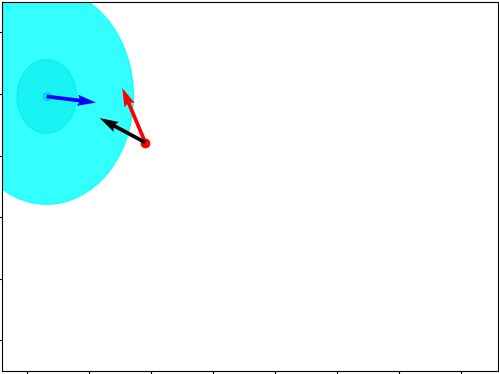
\includegraphics[width=0.95\textwidth]{img/simulation1.png}
  \end{subfigure}
  \begin{subfigure}{0.25\textwidth}
    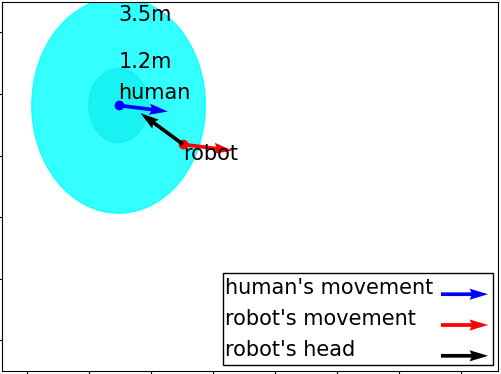
\includegraphics[width=0.95\textwidth]{img/simulation2.png}
  \end{subfigure}
  \begin{subfigure}{0.25\textwidth}
    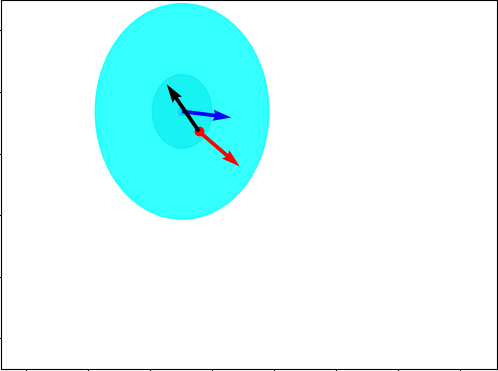
\includegraphics[width=0.95\textwidth]{img/simulation3.png}
  \end{subfigure}
  \begin{subfigure}{0.25\textwidth}
    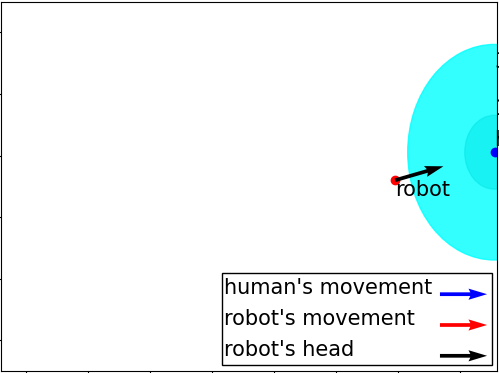
\includegraphics[width=0.95\textwidth]{img/simulation4.png}
  \end{subfigure}
  \caption{ロボットの振る舞い}
  \label{pic:robot}
\end{figure}
まずはじめに半径3.5mの薄青色の円に入るまでは衝突位置にむかってすすむ。その後円内では、人と同じように進むが人の速度がロボットよりも速い場合は
ロボットと人の距離が近くなりすぎる場合がある。そのような時はロボットの向きはそのままに人から遠ざかるように動く。
その後薄青色の円から出た場合は追従をあきらめ立ち止まる。
  \item 移動方法計算 \\
  既存のソフトウェアであり発行されたゴールポーズを目指し障害物を避けながら、robotに対して移動速度、回転速度についての指令を行う。

  \item インターフェース \\
  ロボットに備え付けられたカメラから受け取った画像データをもとにして
  図\ref{pic:interface}のようなインターフェースを作成した。
  インターフェースでは、ゴール計算の際の各人に対して衝突可能かどうかを用いて、
  図\ref{pic:interface}のように衝突可能な人は緑枠で、不可能な人は赤枠で囲むこととしている。
  このインターフェースを用いて、オペレータは
  緑枠に囲まれた歩きスマホをしている人をクリックすることとなる。その際、ターゲットに選ばれた人を囲む枠は太く塗られ、オペレータは今
  だれを追跡しているかについて知ることができる。その後クリックされた人のidをゴール計算に定期的に送る。そこでゴール計算では、そのターゲットidを受け取るたびに
  送られていた人との衝突可能位置をゴールポーズとして発行する。ここでゴールポーズとは目標となる位置と向きのことであり、その向きは
  人の向きであり、ロボットが常に人の方向を見るようにしている。
  また、画面両端にてカメラに写っていない人についての情報を得ることができる。
  これはオペレータが歩きスマホをしている人を
  探す際に常に回転する必要があるという問題の解決のためであり、この機能によってオペレータは左右に人がいる場合にのみ、
  回転を行えばよい。
  \begin{figure}[htbp]
  
    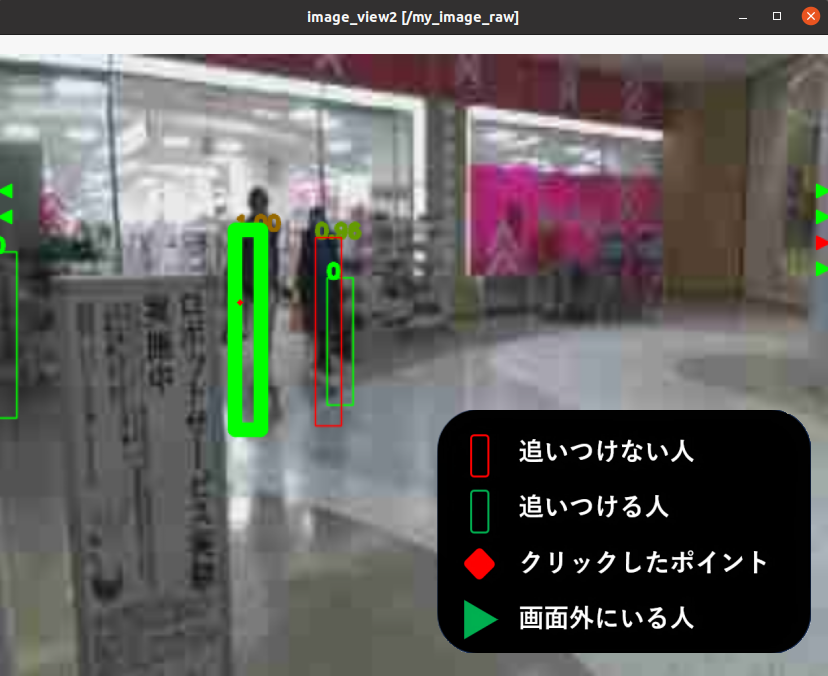
\includegraphics[width=15cm]{img/interface.png}
    \caption{操作支援インターフェース}
    \label{pic:interface}
  \end{figure}
  
\end{itemize}
\vspace{5mm}




%\subsubsection{メディア}
%media部分では、ロボットの備え付けられたカメラのデータ、マイクのデータを取得し、インターフェースに送る。また、オペレータの発した声
%を直接そのままロボットに備え付けられたスピーカーから出力する。


\subsection{有効な注意文言の検討}
認知的不協和理論に基づき、なるべく歩きスマホをやめさせるような注意文言の検討を行う。
一度目の歩きスマホの注意の後も歩きスマホをやめない人は、
注意によって生じた不快感を解消するために、\ref{sec: CDT}章で述べた解消方法の中で「行動を変える」以外のいずれか
を用いていると考えられる。そこでその解消方法に対抗するような文言によって、不快感の解消を困難にすることで
「行動を変える」という選択肢をとらせることが可能になると考える。
\label{sec: dissonance}
\begin{figure}[htbp]
  
  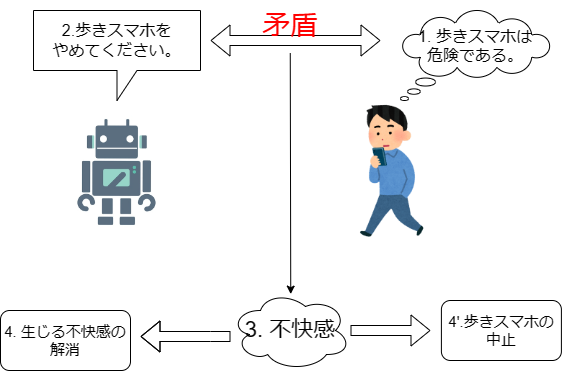
\includegraphics[width=13cm]{img/CDT.png}
  \caption{不快感が生じるまでの流れ}
  \label{fig: dissonance}
\end{figure}
まず多くの人が歩きスマホのことを危険だと考えており、さらに注意された際に不快感が生じることは示されている。
\cite{Schneider2022}では具体的に、人が歩きスマホを注意されたとき図\ref{fig: dissonance}のように、以下のような過程を経ることが示されている。
\begin{itemize}
  \item[(1)] 歩きスマホをしている人も信念として、歩きスマホが危険であるという信念を持っている。
  \item[(2)] ロボットが注意を行う。
  \item[(3)] 自分の行動と信念とが矛盾していることに気付かされ不快感が生じる。
  \item[(4)] 歩きスマホをやめる。
  \item[(4')]歩きスマホをやめる以外の不快感の解消方法をとる。
  \label{item: dissonance}
\end{itemize}
ここで、(4)ではなく(4')の行動を行った相手に対してその解消方法に応じた
追加の注意喚起によって、(4)の行動をとらせることを目指す。歩きスマホを注意された人は
表\ref{fig: UsingPhone}のような認知を持っており、認知1と認知2の矛盾によって不快感が生じる。
\begin{table}[h]
  \centering
  \caption{歩きスマホによる不快感}
  \label{fig: UsingPhone}
  \begin{tabular}{c|c}

      認知1 & 歩きスマホは危険である  \\ \hline
      認知2 & 私は歩きスマホをしている \\ 
  \end{tabular}
\end{table}
\ref{sec: CDT}章で述べたように、注意された人は不快感を解消するためいくつかの選択肢をとることができる。これらの選択肢の内、
行動を変えるという選択肢をとらせることが本システムの目標である。そのために、それ以外の選択肢をとった際にその解消方法を無効にするような文言や、
新たに不快感を生じさせるような文言によって、再度不快感を解消する必要性を生むことで行動を変えるという選択肢をとらせることが可能になると考える。
ここで歩きスマホを注意された人の不快感の解消方法それぞれについて考える。

\begin{enumerate}
  \item 行動を変える \\
 行動を変えることは、歩きスマホをやめることでありこの場合これ以上注意を行う必要はない。

  \item 認知を変える \\
   認知を変えることは、表\ref{fig: UsingPhone}の認知1を「歩きスマホは危険ではない」とすることである。この認知の変更を困難にするためには、
  再度歩きスマホが危険であるような認知を追加するような文言が有効であると考えられる。例えば、
  「歩きスマホによる死亡事故例も存在します」や「歩きスマホによって他人をケガさせた場合、高額の賠償金を請求される可能性があります」
  等があげられる。
  \begin{table}[h]
    \centering
    \caption{認知の変更}
    \label{fig: AvoidDissonanceRevise}
    \begin{tabular}{c|c}
        認知1' & 歩きスマホは危険\sout{である}ではない \\ \hline
        認知2 & 私は歩きスマホをしている \\ \hline
        認知3 & 歩きスマホによる死亡事故が存在する \\
    \end{tabular}
  \end{table}
  そのような注意を受けたとき表\ref{fig: AvoidDissonanceRevise}のように認知3が追加される。
  そして、認知1'と新たに追加された認知3の矛盾により新たに不快感が生じることとなる。
  もしくは、認知1の変更が困難になる。それらの結果として、この方法での不快感の解消が難しく再び不快感の解消を試みなければならない。
  なので、この選択肢がとられた際に有効な
  注意文言は歩きスマホが危険であることを示す文言であると考えられる。

  \item 新たな認知の追加 \\
  不快感の解消のために、表\ref{fig: AvoidDissonance}の認知3や認知4が追加されることが考えられる。これらの認知は、
  認知1と認知2の矛盾を軽減させることができるため不快感の解消につながる。
  \begin{table}[h]
    \centering
    \caption{新たな認知の追加}
    \label{fig: AvoidDissonance}
    \begin{tabular}{c|c}
        認知1 & 歩きスマホは危険である \\ \hline
        認知2 & 私は歩きスマホをしている \\ \hline
        認知3 & 地図アプリを見ており、これは必要な行為である \\\hline
        認知4 & 周りに人がおらず、他人に迷惑をかけていない \\ 
    \end{tabular}
    
  \end{table}
  そこで、これらの認知の追加に対しては、認知3の追加に対して「道案内なら私がしますよ。」や認知4の追加に対して
  「そこの柱の裏から急に人が飛び出してくるかもしれません」といった文言が有効であると考えられる。
  \begin{table}[h]
    \centering
    \caption{新たな認知の追加}
    \label{fig: AvoidDissonanceBlock}
  
    \begin{tabular}{c|c}
        認知1 & 歩きスマホは危険である \\ \hline
        認知2 & 私は歩きスマホをしている \\ \hline
        認知3 & 地図アプリを見ており、これは必要な行為である \\
        認知3' & 道案内を目の前の人に頼むことができる \\ \hline
        認知4 & 周りに人がおらず、他人に迷惑をかけていない \\ 
        認知4' & そこの柱の裏から急に人が飛び出してくるかもしれない \\ 
    \end{tabular}
    
  \end{table}
  これらの
  文言は追加される認知と矛盾するものであり、図\ref{fig: AvoidDissonanceBlock}のように認知3と認知3'の矛盾を生じさせることで
  新たな不快感が生まれる、もしくは、認知3の追加を防ぐことができると予想され、結果として注意された人は再び不快感の解消を試みなければならない。
  よってこの選択肢がとられた際に有効な注意文言は、追加された認知に対して矛盾する文言であると考えられる。
  \item 矛盾の矮小化、無視 \\
  ロボットが矮小化や無視の対象となることが多い\cite{Schneider2022}。そのためこの選択肢がとられた際には、
再度ロボットを無視することが困難になるような文言が有効であると考えられる。
これは対象の外見の特徴を述べたうえで注意することによって、ロボットの矮小化を防ぐことができると考えられる。
具体例として考えられる会話の例を表\ref{dialogue: Ignore}に示した。
\begin{table}[H]
  \centering
  \caption{矮小化・無視}
  \label{dialogue: Ignore}
  \begin{tabular}{c|c}
      ロボット & 歩きスマホは危険ですので、おやめください。 \\ \hline
      人 & (無視) \\ \hline
      ロボット & そこの青いシャツを着ている方に言っています。 \\ 
  \end{tabular}
  
\end{table}
\end{enumerate}
\vspace{5mm}
以上の考察から、どのような時にどのような文言が有効であると考えられるかについてを
表\ref{fig: EffectiveWords}にまとめた。
\begin{table}[H]
  \centering
  \caption{有効な注意文言}
  \label{fig: EffectiveWords}
  \begin{tabular}{c|c|c|c}
      \multicolumn{2}{c|}{選択肢} & \multicolumn{2}{c}{有効な注意文言} \\ \hline
      \multicolumn{2}{c|}{行動を変える} & \multicolumn{2}{c}{-} \\ \hline
      \multicolumn{2}{c|}{認知を変える} & \multicolumn{2}{c}{歩きスマホは危険であることを強調するもの} \\ \hline
      \multicolumn{2}{c|}{新たな認知の追加} & \multicolumn{2}{c}{追加された認知に矛盾する文言} \\ \hline
      \multicolumn{2}{c|}{矛盾の矮小化、無視} & \multicolumn{2}{c}{対象の外見の特徴を述べた文言} \\
  \end{tabular}
\end{table}
\section{実験}
\subsection{実験目的}
現段階では具体的にどのような状況に対してどのような文言が有効であるかは不明である。そこで
この実験では注意文言提示システムの構築のために、どのような行動がどの解消方法を意味するかを調べることを目的とする。
実験では歩きスマホをしている人に対して、用意した文言のいずれかを用いて注意喚起を行い、その後の行動を記録する。

\subsection{実験方法}
警備員の格好をしたアバターロボットを用い、大型のショッピングモールであるATC\footnote{https://www.atc-co.com/}の中で、歩きスマホをしている参加者に対して注意喚起を行った。また注意喚起の際に、アバターロボットを操作するためのインターフェースを用いた。
実験の様子を図\ref{fig: Experiment}に示す。
\begin{figure}[H]
  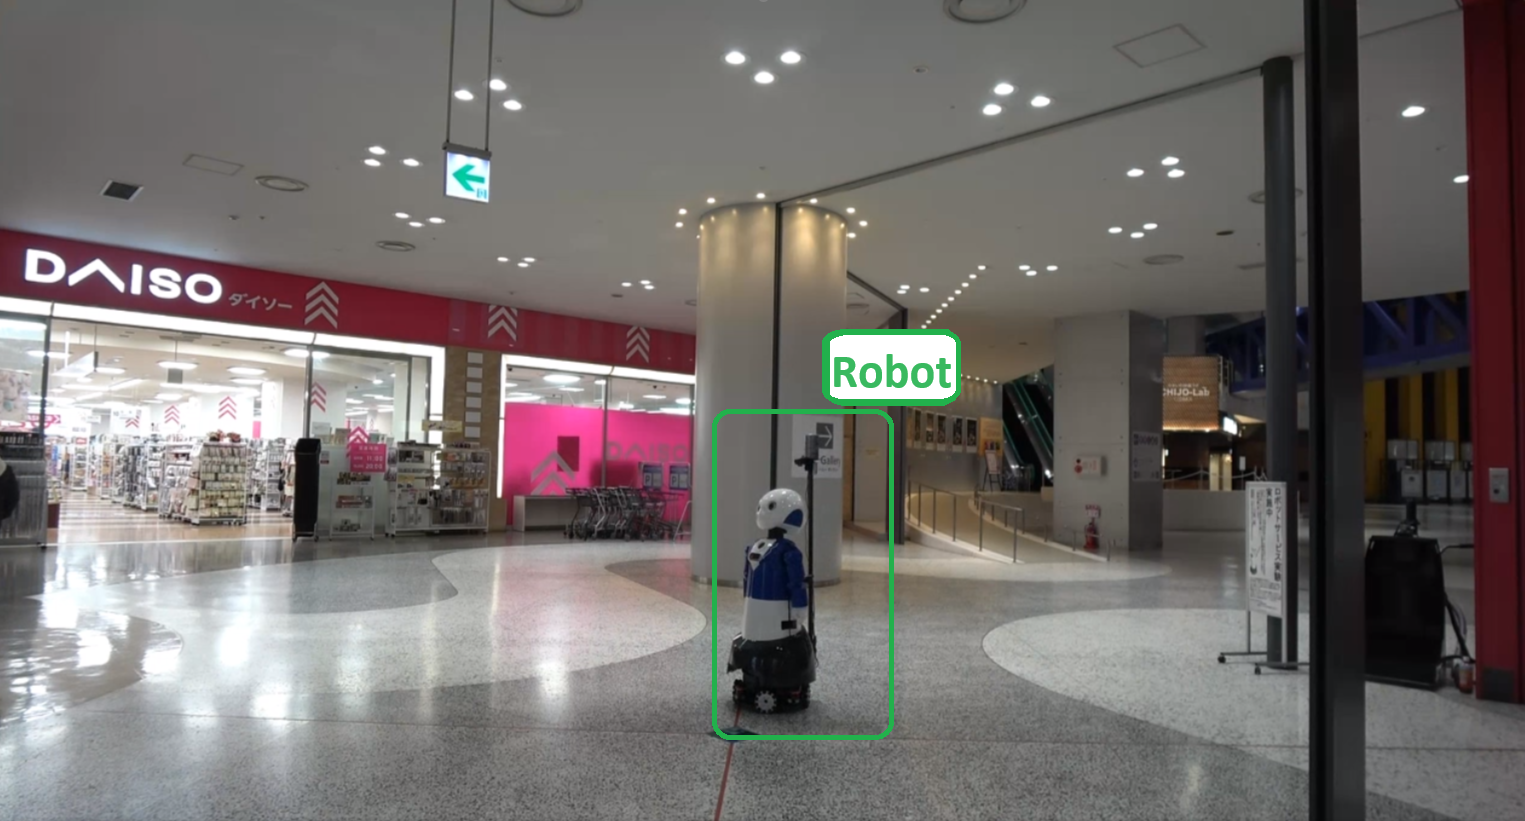
\includegraphics[width=15cm]{img/Experiment.png}
  \caption{実験環境}
  \label{fig: Experiment}
\end{figure}

用いた注意文言は図\ref{fig: Strategy}の通りである。
\begin{figure}[h]
  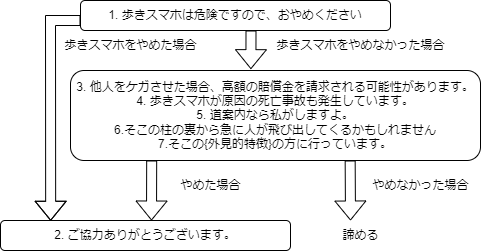
\includegraphics[width=15cm]{img/waystostop.drawio.png}
  \caption{注意文言}
  \label{fig: Strategy}
\end{figure}
実験の手順は次のように行った。
\begin{enumerate}
  \item 用意したインターフェースを用いて歩きスマホをしている人に近づく。
  \item 全ての人に対して、「歩きスマホは危険ですのでおやめください。」という注意喚起を行う。
  \item 歩きスマホをやめなかった場合、反応から最も適切だと思う図\ref{fig: Strategy}の注意文言3,4,5,6,7のうち一つ選択し再度注意喚起を行う。
  \item その後、歩きスマホをやめたかどうかを記録する。
\end{enumerate}


\subsection{実験参加者}
今回の実験では、実験協力者として計7組に対して注意を行った。そのうち2組は事前に協力をお願いしてロボットの前で歩きスマホをしてもらい、
さらに1度目の注意を無視するようにお願いした。
残りの5組は実験当日にロボットの近くで歩きスマホをしていたATCへの来場者であった。
\subsection{実験結果}
事前協力者には図\ref{fig: Strategy}における文言3,4,5,6,7の5種類の注意文言を用いて1回ずつ計5回注意を行った。
以下図\ref{fig: Experimentjani}, 図\ref{fig: Experimentjani2}に注意の様子を示す。
\begin{figure}[h]
  \begin{subfigure}{0.5\textwidth}
    \centering
    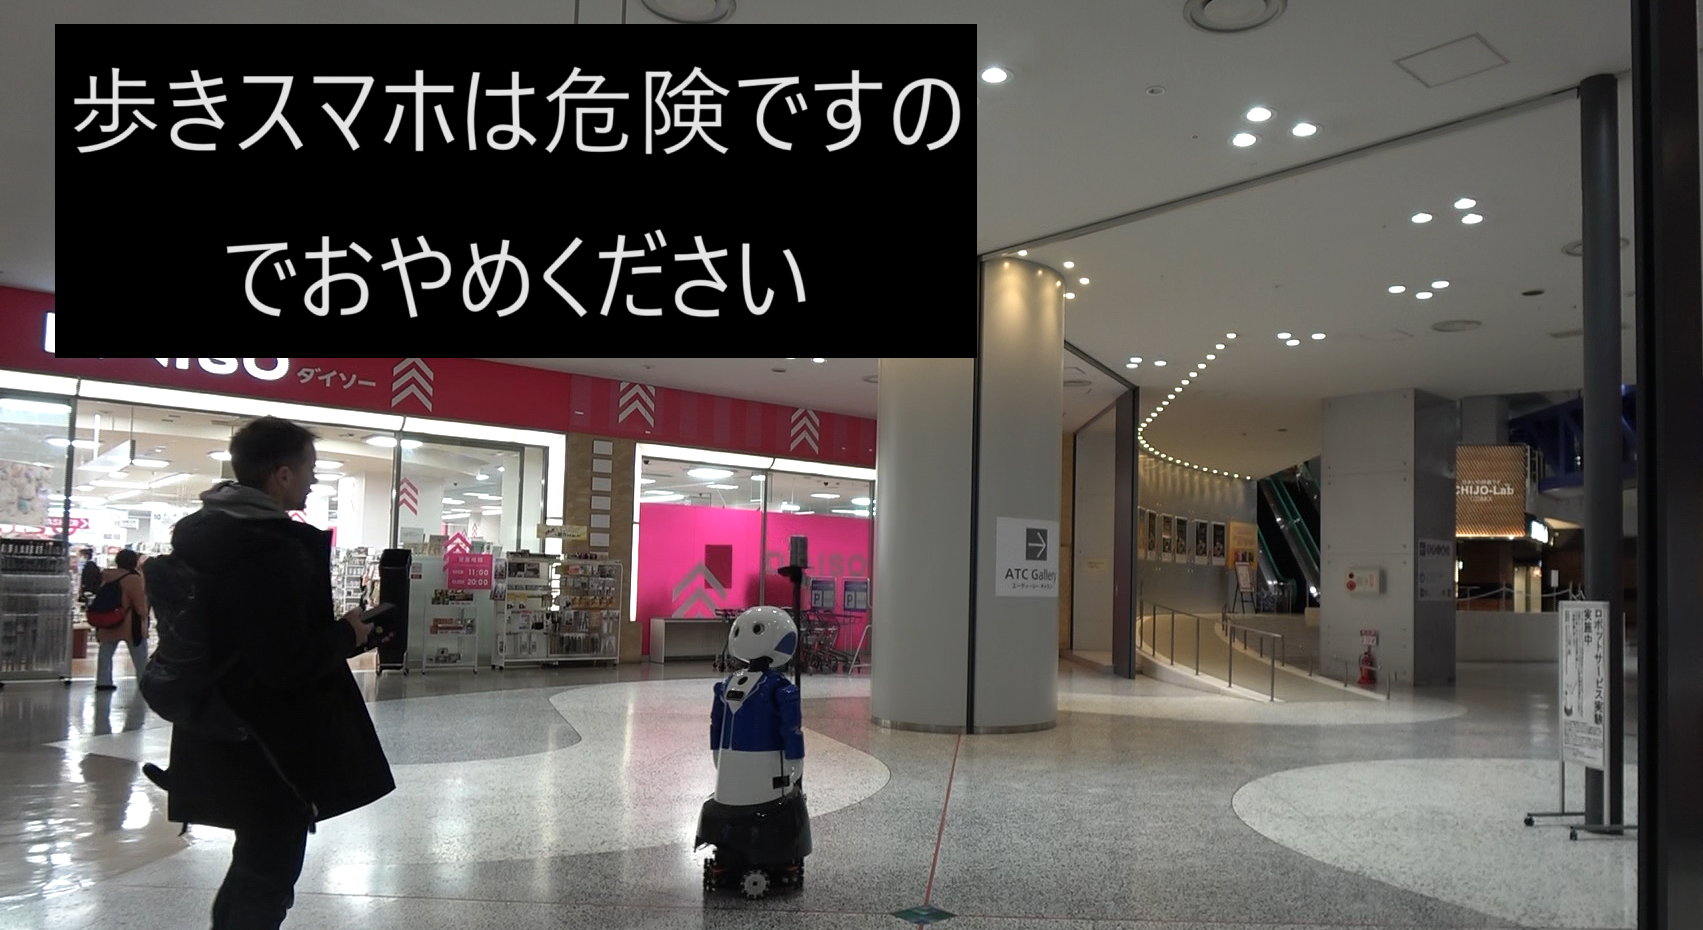
\includegraphics[width=0.95\textwidth]{img/jani2.png}
    \caption{実験の様子1}
    \label{fig: Experimentjani}
  \end{subfigure}
  \begin{subfigure}{0.5\textwidth}
    \centering
    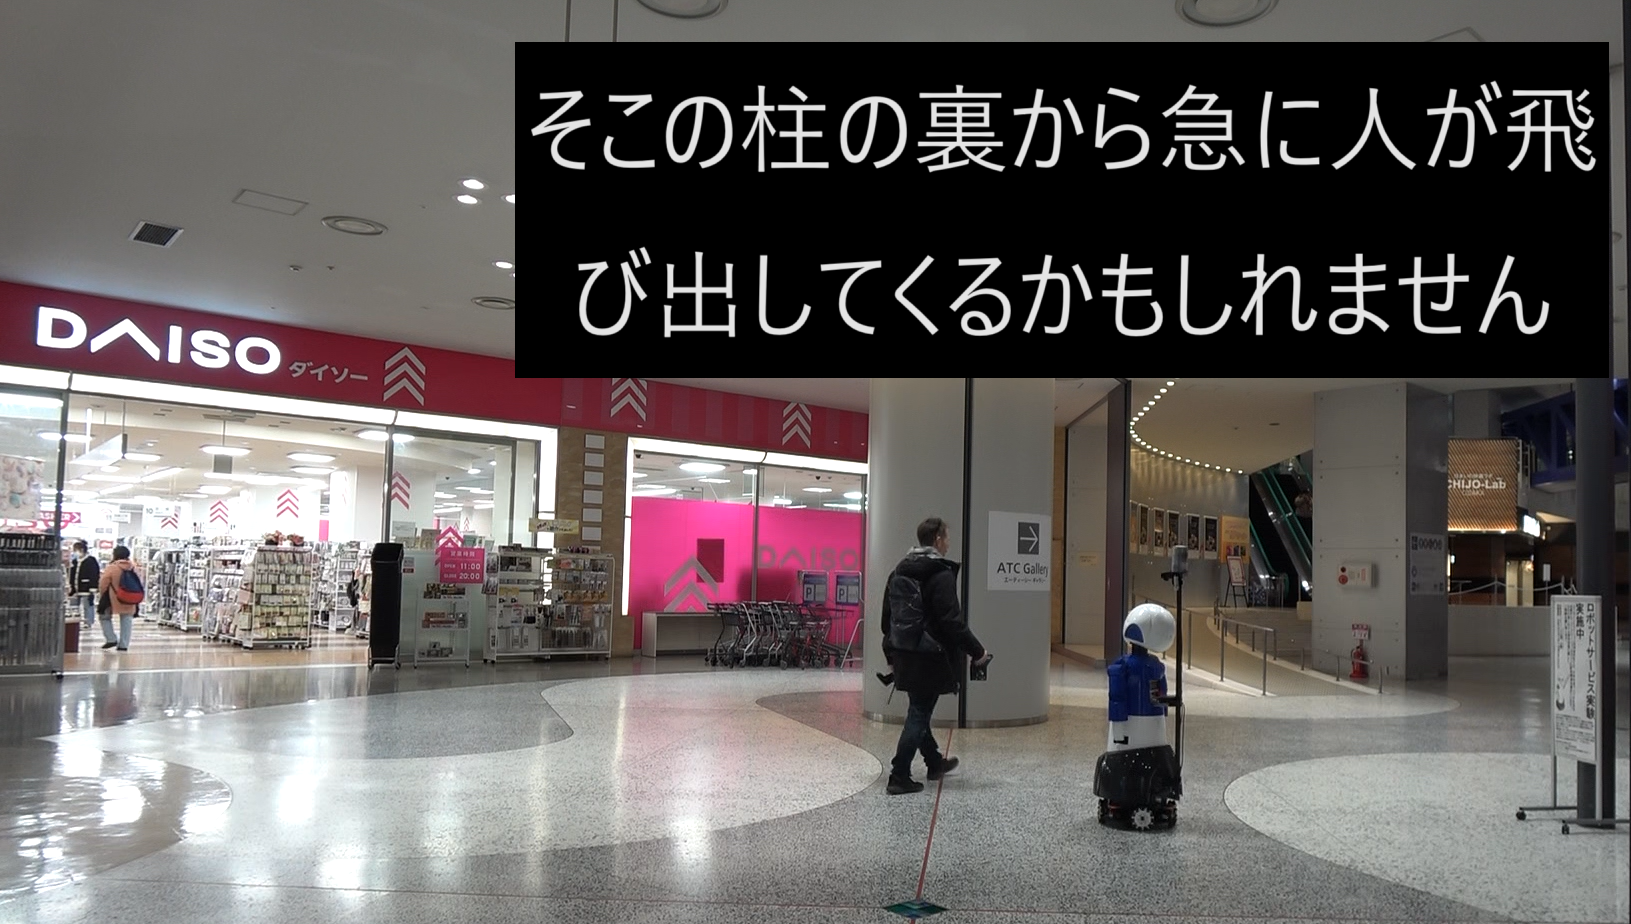
\includegraphics[width=0.95\textwidth]{img/jani3.png}
    \caption{実験の様子2}
    \label{fig: Experimentjani2}
  \end{subfigure}
\end{figure}
その後のインタビューでは次のような意見が得られた。
\begin{itemize}
  \item 容姿の特徴を述べる注意文言用いた時に、自分が特定されていることで孤立感を感じ無視することが難しかった。
        また容姿の特徴を述べることによって周囲の人間の注目を集め、無視した際に周囲の人間からの怪訝なまなざしを向けられることも無視しづらい要因であった。
  \item 歩きスマホの危険性を強調する注意文言では、抑止力はかなり弱かった。
  \item 自分がロボットに注意されるのを目撃した他の歩きスマホをしている人は、歩くのをやめてその場で立ち止まって携帯を触っていた。
  \item ユーモアを用いるのも有効だと思った。
\end{itemize}

また残りの5組に関して注意した状況、どのような注意文言を用いたかそして結果はどうであったかについて
説明を行う。一度目の注意はいずれも「歩きスマホは危険ですのでおやめください。」という文言を用いた。
\begin{enumerate}
  \item[Case1] 男性1人でスーツを着用しており、歩行速度はかなり早めであった。一度目の注意ではこちらのほうに視線を向けることなく歩きスマホを継続した。その後、
  「そこの柱の裏から急に人が飛び出してくるかもしれません」
  と注意したが、話しかけ始める時点が遅かったため、相手の後方から話すこととなり無視され歩きスマホを止めることはできなかった。
  \item[Case2] 女性2人組で片方が歩きスマホをしており、歩行速度は遅めであった。一度目の注意をおこなったところ、
  ロボットの方向に近づいきた。その後、「道案内なら私がしますよ」と話すと、
  「駅の方に行きたいです」と返答があったため、その方向を指し示した。その後歩きスマホをやめたがスマホは手に持ったままであった。
  \item[Case3] 男性1人で平均的な速度であった。一度目の注意に対して、英語で「私は中国人なので中国語で話して」と返答があったため、
  中国語を話せる人にオペレータを代わってもらい、中国語で注意を行ったところロボットを凝視したのちに歩きスマホをやめ歩行を再開したが、
  その後しばらくの間もロボットを見ていた。
  \item[Case4] 男性1人で歩行速度はかなり遅めであった。1度目の注意でこちらに少し目を向け歩きスマホをやめ歩行速度を速めた。そのため
  2度目の注意は行わなかったが、実際はしばらくしたのちに歩きスマホを再開していたが、オペレータはそのことに気づかなかった。
  \item[Case5] 男女複数名のグループで全員スーツを着用しており、そのうち1人の女性が歩きスマホをしていた。グループ全体の歩行速度は平均的であった。
  一度目の注意で歩きスマホをやめ、それ以上の注意は行わなかった。その後グループの何人かがロボットのほうを見て
  ロボットについて話をしていた。
\end{enumerate}
特にCase2の様子を図\ref{fig: Case3}に示す。
\begin{figure}[H]
  \centering
  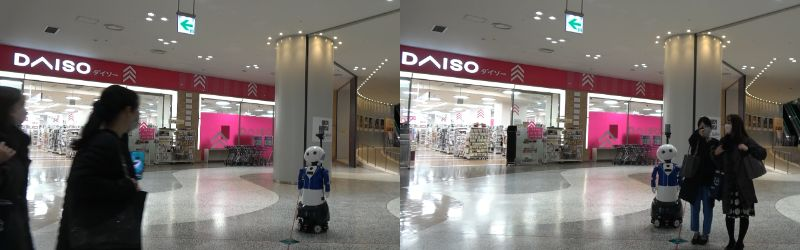
\includegraphics[width=15cm]{img/Case3.jpg}
  \caption{Case2}
  \label{fig: Case3}
\end{figure}

\subsection{実験結果の考察}
実験での観察から解消方法の識別に重要な属性として、周囲の状況、歩行速度、恰好、
グループの人数、注意された際の反応があると考えられた。
例えばスーツを着用している人は普段からATCを利用している人が多いと考えられるため、地図アプリを見ている可能性は低い。
しかしCase2のように歩行速度が遅い場合、地図アプリを利用している可能性が高く「道案内なら私がしますよ」という文言が有効になる。
またやめなかった人に共通する特徴として、ロボットに対して興味を抱いていなかったことがあげられる。
歩きスマホをやめたCase2, Case5, Case3では、いずれもロボットに興味を示すそぶりを見せていた一方で、
歩きスマホを最後まで継続していたCase1, 4ではロボット対してそれほど目線を向けることがなく、
ロボットに対して興味を示していなかった。
Case3では用意した文言以外を用いることになったが歩きスマホをやめた理由として、
唐突に中国語で話すことで相手に強い驚きを与えられたことが考えられる。
実際Case3では歩きスマホをやめたあとも、
しばらくの間ロボットの方向を見ながら歩いていた。


またアンケートからは周囲の人から注目されている時には無視することが難しいという意見が得られた。
これは不快感の解消のために歩きスマホをやめたのではなく、周囲の人々の同調圧力から歩きスマホをやめたと考えられる。
また歩きスマホの危険性を強調する文言の抑止力が弱いという意見が得られたが、
これは無視するようにお願いしているため「実験のために歩きスマホをしている」という認知が追加されており、
不快感が生じなかったことが原因と考えられる。

これらの結果から解消方法の識別に必要な属性として、周囲の状況、歩行速度、恰好、グループの人数、注意された際の反応があると考えられる。
ほかにもユーモアや驚きを与えることで相手に強い印象を与えることでロボットを無視しづらい存在にする戦略や、
同調圧力を用いた戦略が有効であることが示唆された。

\section{今後の課題}
今回の実験では注意文言の中からどのような解消方法をとられたかどうかに基づいて注意文言の選択を行ったが、
それでは認知的不協和理論について詳しくない人にとっては、それを判断し注意文言を選択することは難しい。
そこでグループの人数や恰好といった誰にとってもわかりやすい属性を用いて、
注意文言の選択を行うことができるような提示システムを作成する必要がある。
今回解消方法の判断において重要であろうと考えられる属性をいくつか見つけることができたが、
それらの属性の値によってどのような解消方法がとられたかを明確にすることはできていない。
そのため今後実験によってそれらの属性の値から解消方法を予測するようなモデルを構築することが必要である。
不協和を利用した戦略以外にも、実験から考えられたユーモアや驚きを用いた戦略や同調圧力を用いた戦略
についての検証も必要である。

移動に関して今回のシステムでは単純に歩きスマホをしている人に一直線に近づくというものであったが、
\cite{Mizumaru2019}のように工夫した近づき方を行うことで、より注意をひきつけることができると考える。




\section{まとめ}
本研究では、警備員の業務の中で歩きスマホの注意を支援するシステムの実装を行った。
第一にコントローラーを用いて歩きスマホをしている人に近づき、継続的にその人の方向を向いているという操作は
困難なものであったため、それらを解決するインターフェースおよびシステムの構築を行った。
第二に認知的不協和理論に基づき、注意されたときに生じる不快感を行動をやめる以外の方法によっても解消できることに着目し、
それらの解消方法に対抗するような文言を考えた。しかし今のままでは、注意文言の選択に認知的不協和理論に関する知識や
どのような行動の時どのような解消方法がとられているかといった情報が必要となるため、注意文言の選択を行うことが難しい。
そこで第三に、解消方法の識別に必要な情報を得るための実験を行った。その結果として、
いくつかの属性が解消方法の識別に重要であるや提案したもの以外の有効な注意文言が考えられることがわかった。
将来課題として
これらの属性を用いた解消方法の予測モデルの構築を行い、それを用い有効な注意文言の提示を行うシステムの構築や
その他の戦略を取り入れることがあげられる。

%=====================================================================================
\acknowledgments %章を付けずにタイトル表示
本研究を行うにあたりご指導頂いた指導教員の神田崇行教授と Jani Even
特定講師、今回の研究の予備実験を手伝ってくださった研究室の先輩、
友人たち、そして実験を行うに当たって協力頂いたATRの方々と実験に協力してくださったATCの来客者の方々
に深い感謝の気持ちとお礼を申し上げ
ます。

%=====================================================================================
\nocite{*}
\bibliography{citation} %bibtexファイルの読み込み
\bibliographystyle{kuisunsrt} %本文に\cite{}を入れることで,参考文献表示

\end{document}